% the school's class loads a font package that announces its own patches; they're harmless
\RequirePackage{silence}
\WarningsOff[nfssext-cfr]

\documentclass{ntu-fyp-report}

\usepackage{xfrac}
\newcommand{\figurescale}{0.85} % every figure is included at this size, so they all look consistent
\usepackage[breakable]{tcolorbox}

% inline code: type underscores and the like as-is, e.g. \code{std::unordered_map}
\newcommand{\code}[1]{\texttt{\detokenize{#1}}}

% let a line stretch a little further rather than push a long \code{} word into the margin
\setlength{\emergencystretch}{3em}

% side notes for the curious: \begin{aside} ... \end{aside}
\newtcolorbox{aside}{
  breakable,
  colback=black!4, colframe=black,
  boxrule=0.6pt, arc=0pt, left=8pt, right=8pt, top=6pt, bottom=6pt,
  before skip=12pt, after skip=12pt,
  before upper={\setlength{\parskip}{0.6em}},
}

\author{Author}
\title{Pushing the Quadratic Boundary when Computing a Closest Pair}

\supervisor{}
\examiner{}

\project{CCDS\,00-0000}
\school{College of Computing and Data Science}
\schoolyear{2026}

\begin{document}

\pagenumbering{roman}

\maketitle

% !TeX root = main.tex

\chapter*{Abstract}

% !TeX root = main.tex

\chapter*{Acknowledgements}


\tableofcontents
\listoffigures

\cleardoublepage
\pagenumbering{arabic}
\setcounter{page}{1}

% !TeX root = main.tex

\chapter{Introduction}

Computing the distance between two points is a common geometrical task.
A natural extension to that would be to find the \textit{closest pair} of points,
i.e., the pair that yields the smallest distance. Assuming a point in $d$-dimensional
space, computing the distance between two points takes $\mathcal{O}(d)$ time.
There are $\binom{n}{2}$ pairs to check, forcing a total time complexity of
$\mathcal{O}(d \cdot n^{2})$.

In general, for large $d$, it's not possible to beat quadratic time in the \textit{worst case}, assuming the
\textbf{Strong Exponential Time Hypothesis (SETH)}. Luckily for us, there are tricks to salvage
the situation at low dimensions, and for practical applications like vector databases,
people have ditched the intractable task of obtaining an exact solution, opting for
approximate algorithms instead.

\section{Duplicate Points}

Depending on the circumstances in which these points were generated, it's quite possible that we
end up with duplicate points. For example, consider the Birthday Paradox. While it seems strange
that only $23$ people are required to produce a coin flip chance of having a shared birthday
(the equivalent of two overlapping points), that's just how the probability checks out.

One way to solve this problem would be to first sort the points and check adjacent items to see if
they're equal. Another approach is to inject them into a \textit{hash set} one by one, and prior to the
insertion, if the set already contains the point, we know a duplicate exists. The extra logarithmic
factor in the former might seem burdensome, but it might actually beat the latter in terms of real
runtime, considering hash sets in many languages are often plagued by high constant factors. Not to
mention sorting also happens to be the first step in many of the subsequent algorithms, so the duplicate
check arrives almost free in a sense.

\section{Points on a Line (\texorpdfstring{$d=1$}{d = 1})}

At $d=1$, the points are just an array $a$ of scalar values, so one may simply sort $a$ and
compare adjacent elements, consuming
$\mathcal{O}(n \log n)$ time. If the range of values ($k = \max(a) - \min(a)$)
is small enough, \textit{counting sort} may be exploited to solve the problem
in $\mathcal{O}(n + k)$.

At this juncture, it's natural to question if it's possible to achieve $\mathcal{O}(n)$
irrespective of $k$, and as it turns out, there are randomised
algorithms with linear expected time. These algorithms are rooted in
the idea of \textit{decomposition}, and they generalise to higher dimensions as well.
We'll elaborate more on the details when we get there.

% !TeX root = main.tex

\chapter{Methodology}

\section{Language Choice}

The algorithms are implemented and tested in C\texttt{++} for several reasons.

\begin{itemize}
    \item A low-level compiled language gives you realistic estimates on how fast these algorithms
    actually are when they aren't held back by overheads like an interpreter.
    \item You get precise control over memory layouts and whether things go on the stack or the
    heap. For the most part, data structures like \texttt{std::array} are preferred because
    they reduce pointer chasing and are more cache-friendly.
    \item Multithreading is easy to perform in C\texttt{++}, thanks to tools like \texttt{std::jthread}.
    Although theoretical time complexities are important, whether or not an algorithm is practical
    and useful in real life also depends on how well it may be \textit{parallelised}.
\end{itemize}

\begin{aside}
    Brute force might be an \textit{embarrassingly parallel} algorithm, but it's still easy to write
    a suboptimal implementation. With $n$ points and $t$ threads, one might think to split
    the points into contiguous chunks of $\sfrac{n}{t}$ points each. The issue is that for the
    points $p_{i}$ at the start, we have to match them with $p_{j}$, where $i < j$, and at
    say $i = 0$, we check a huge number of points, whereas for a late $i$, there's nothing much to check.
    Thus, the thread in charge of the first block bears a lot more work, and takes longer to finish.

    To improve the distribution of work, let's implement a rule where point $i$ is handled by thread
    $i \bmod t$. Each thread has its own local best, and at the end, we update the global pair
    based on these local pairs. One advantage to this technique is that we avoid having to use
    synchronisation primitives like atomics or mutexes (which add extra overhead) to protect the global
    answer from race conditions.
\end{aside}

\begin{aside}
    You may get the thread count using \code{std::thread::hardware_concurrency()}. On my machine
    that's twelve threads. Unfortunately, this doesn't imply that we'll get a twelvefold speedup,
    since the processor consists of both performance cores and efficiency cores, with the latter running
    at only a fraction of the speed.
\end{aside}

\section{Point Generation}

A meaningful dataset should try and avoid degenerate cases like duplicate points. This
necessarily forces a large-enough range to circumvent the Birthday Paradox. In addition,
it should be easy to compute the distance between any two points, and compare distances
accurately. In other words, let's avoid floating point operations. Not only is it easy to mess up
comparisons, when adding floats together the ideal strategy is to sort them by size and add
the smallest numbers first before merging with the large ones. And this adds extra overhead
that detracts from the core task at hand.

So \texttt{int} it is, and because we're working with \textit{Euclidean} distances, a trick
to preserve precision and reduce operations is to avoid the square root altogether, and
compare squared distances instead. To spawn a set of points, we used the \textit{Mersenne Twister}
pseudorandom number generator (\code{std::mt19937_64}) to achieve a uniform random distribution
of points. Fixed seeds are also used to ensure fair benchmarking.

\section{Correctness Checks}

As we implement various (increasingly complicated) algorithms, it's essential to validate
their correctness. The simplest way to do so is to use the brute-force algorithm as
a baseline, and check if the squared distance (conveniently, an integer) between the
closest pair is the same across a range of different test cases. From my personal
experience, here are some common mistakes and pitfalls.

\begin{itemize}
    \item You get a best distance of \textit{zero}, even though brute force produced a nonzero value.
    This is likely because in the inner loop, you wrote \code{int j = i}, instead of \code{int j = i + 1},
    so you mistakenly used the same point twice.
    \item You did not achieve the best distance. This might be because you failed to enumerate neighbours
    correctly (e.g., during grid decomposition), or you messed up the base case in recursive algorithms
    such as divide-and-conquer.
    \item Strange and inconsistent behaviour across different runs. This might be a symptom of
    \textit{undefined behaviour}, and the cause is usually out-of-bounds access, a data race (during
    multithreading), or signed overflow.
\end{itemize}

\section{Benchmarking}

To figure out which algorithms are ``better'' than others, the most practical approach
is to measure their runtimes. There are some ground rules we set to provide the fairest
comparison. First, point generation should never be considered as part of runtime; we'll
always generate them before starting the clock. Next, points are fed to the solver by
\textit{value}, not reference. Algorithms are free to mess with the dataset however they like,
with the original dataset remaining unaffected. Third, you pay for the cost of building data
structures, assuming you need one (e.g., grid decomposition). As long as meaningful work is being
done to contribute to the solution, we feel that it should add to the measured runtime. Finally, fixed seeds
are used to generate the datasets, ensuring replicable results.

Figure~\ref{fig:methodology_benchmark_pipeline} illustrates the benchmark pipeline in full detail. Everything
begins with a TOML file. Instead of handwriting loops and conditional statements in \code{main.cpp}, we
abstract this process away through the \code{config.toml} file. You only need to specify information like
the algorithms of interest, the sizes of the dataset, dimensions, trial counts, and other auxiliary information.
Compile just once, and tweak \code{config.toml} from there on. For consistency, unless specified otherwise,
we always run thirty trials (i.e., samples) throughout all experiments in this paper. This helps even out
the effects of a super lucky or unlucky run. The settings are checked before anything runs, and any problems produce
explicit errors, so you can fix issues right away instead of discovering something broke an hour
into a run.

There are two kinds of seeds: a dataset seed that decides the points, and a solver seed that controls a
solver's random choices (think randomised algorithms). Each of these seeds is created from a base seed ($42$),
mixed with $n$, $d$, $t$ (trial number), and a label. We always make sure to reset the solver seed so
the order in which the algorithms are specified does not matter.

Only the lime section is measured; things like creating the dataset or copying the points should not count
towards an algorithm's performance. After all iterations are completed, the results are written back to disk.
A run that fails halfway (which is very unlikely to happen anyway) or stops early loses all progress, but in
a sense the all-or-nothing, atomic behaviour also has its charm.

Because of the nature of the benchmark, ratios and normalised scores repeat \textit{exactly} between
runs. Sadly, runtimes do not enjoy this repeatability, because they depend on the machine, and even
on the same machine, the presence of other processes can interfere with the effectiveness of techniques
like multithreading.

\begin{figure}[ht]
    \centering
    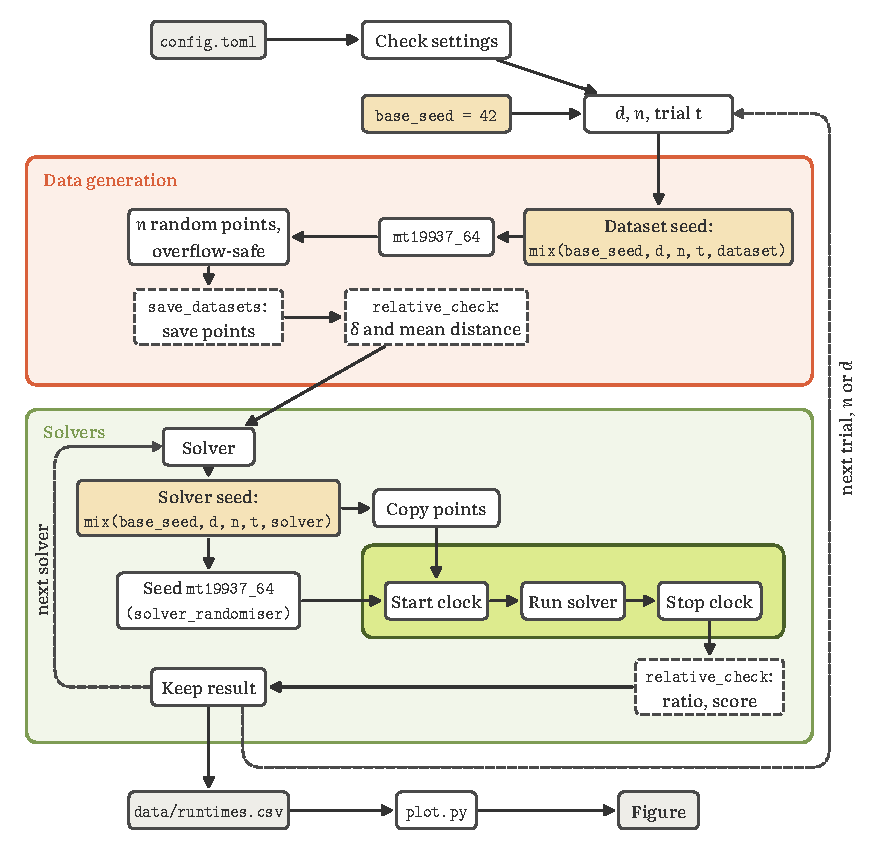
\includegraphics[scale=\figurescale]{diagrams/methodology_benchmark_pipeline.pdf}
    \caption{How one benchmark runs. The seeds (in yellow) all originate from one base seed, so every
        solver in a trial gets the same points and the same starting randomness, regardless of the
        order that solvers run in. Dashed boxes only happen if the config asks for them.
    }
    \label{fig:methodology_benchmark_pipeline}
\end{figure}

% !TeX root = main.tex

\chapter{Low Dimensions}

\section{Two-dimensional Points ($d=2$)}

Numerous works have explored the two-dimensional case, and there exist well-known
$\mathcal{O}(n \log n)$ solutions. Perhaps the most famous one is through divide-and-conquer,
so let's begin with that.

\subsection{Divide-and-conquer}

Let's divide the set of points into two (approximately equal) halves. If $n$ is odd, the
first set will just be of size $\lceil \sfrac{n}{2} \rceil$ and the second set will
be of size $\lfloor \sfrac{n}{2} \rfloor$. Intuitively, we want those with smaller $x$
in one set and those with larger $x$ in the other. For convenience, we can sort the
points beforehand, with the sorting key being the point vector itself, i.e., perform element-wise
comparison (check who has the smaller $x$, else if they have equal $x$, compare by $y$ instead).

In the base case of $n = 1$ we simply return infinity (there's no pair!), else let's assume we have solutions to
both halves. Let's take the minimum answer from each half (we'll denote this distance $\delta$).
Our goal is to potentially connect points from the two sets to achieve a new minimum. Consider the
vertical divider ($x = x_{\text{mid}}$) used to partition the halves. Our candidate points are going to lie in the interval
$(x_{\text{mid}} - \delta, x_{\text{mid}} + \delta)$. For some point $(x_{0}, y_{0})$ in this set, we may check just those in the
interval $y \in (y_{0}-\delta, y_{0} + \delta)$. In fact we may just check those points with $y \leq y_{0}$,
avoiding duplicate work.

This ``box'' of width $2 \cdot \delta$ and height $\delta$ contains $\mathcal{O}(1)$ points. Consider
the left and right squares composing this box. If we partitioned each square into a grid of four smaller
sub-squares of width $\sfrac{\delta}{2}$, you may fit at most one point into each sub-square. Even
if we had placed points as far apart as possible, the distance is still $\sfrac{\delta}{\sqrt{2}}$.
If two points fitted in a sub-square, that'll imply we should have gotten a smaller answer
from one of the sub-problems, producing a contradiction.

To check points in this box easily, we'd like the points to be sorted by the $y$ coordinate instead.
This can be done exactly like how you'd perform \textit{Merge Sort}. Surprisingly, the nature
of our divide-and-conquer approach is no different from that of Merge Sort, and our time complexity
is hence $\mathcal{O}(n \log n)$.

\begin{aside}
    Parallelising this algorithm is nontrivial, which is why we opted out of it. While it seems plausible
    to assign a new thread to solve each subtree, we end up with way too many threads (in the order of $\mathcal{O}(n)$),
    and the overhead costs of creating a thread (e.g., reserving a new stack) slow down the system far more
    than any potential savings. Of course, a smarter solution would opt for tools like
    thread pools to keep the thread count manageable, but figuring out the right allocation is pretty tricky as well.
\end{aside}

\subsection{Sweepline}

One downside of divide-and-conquer is the runtime overhead of the recursive calls. An alternative
that yields the same time complexity (and also happens to be a bit faster empirically) is
a sweepline approach. We begin by sorting the points like in divide-and-conquer. Next, we'll
iterate through the points, and maintain a set of earlier points. This set organises the points
in terms of $y$ values.

Given the current minimum distance $\delta$ and the current
point $(x_{0}, y_{0})$, we only need to check points in the set with $y \in (y_{0} - \delta, y_{0} + \delta)$.
Using a similar box analogy, one may prove we check a constant number of points, producing an
overall complexity of $\mathcal{O}(n \log n)$. Implementation-wise, we use C\texttt{++}'s
\texttt{std::set} that uses a balanced binary search tree (specifically a red-black tree) under the hood.

\begin{aside}
    Because of the sequential nature of the sweep, it's not easy to parallelise this algorithm
    either. We require the rolling set of points sorted by $y$, and it's not feasible to have
    some sort of shared set across independent sweeps.
\end{aside}

\subsection{Grid Decomposition}

As alluded to at the start, there are algorithms that offer linear expected time. The trick is
to visualise the search space as a grid, and group points into squares on a grid. To figure
out the nearest pair, there are two cases to handle. First, iterate all pairs within
a grid square. Second, considering a point within a square, let's check its distance
against all other points in adjacent squares. If we pick a good grid width, we'll only
run through a constant number of pair checks per grid square, thus yielding $\mathcal{O}(n)$ time.

Intuitively, the grid width should be neither too big nor too small. A grid that's too fine-grained
might make it impossible to find a neighbouring point in the vicinity, and a large grid width
just degenerates into the brute force search. In a perfect world, we'd take the distance between
the closest pair as the grid width, but that brings us right back to the original problem. Eventually,
people discovered that taking the minimum distance of a bunch of random points (i.e., sample $n$ pairs)
produces a grid width that works surprisingly well.

The first version of the randomised grid approach was actually proposed by Rabin~\cite{rabin1976} half
a century ago. In this version, he sampled about $\sqrt{n}$ points
and took the distances produced by these points. This takes only $\mathcal{O}(n)$ time! He
also proved that it runs in linear expected time. Many years later, it was Lipton~\cite{lipton2010}
who discovered sampling random pairs worked too, and it made the analysis much easier (because each sampled distance
is independent of the others).

Implementation-wise, we use the \textbf{SplitMix64} hash function paired with a hash map. At
the moment we settled with the standard library's \code{std::unordered_map}. Despite
the amortised $\mathcal{O}(1)$ lookup, its closed addressing scheme isn't particularly
cache-friendly.

\begin{aside}
    Finally, we have a nontrivial algorithm that's worth multithreading. Unlike brute force,
    where we made each thread responsible for a set of points, this time let's have each
    thread take charge of a set of squares instead. As usual, we'll allocate a roughly 
    equal number of squares to each thread. Since viewing points in neighbouring squares
    is a read-only operation, we don't need to guard it from data races. One implementation
    detail is to extract all the iterators beforehand, and not to be misled by
    the sneaky \code{std::views::stride(t)} (it doesn't allow for a random access jump when
    iterating over \code{std::unordered_map}).
\end{aside}

Figure~\ref{fig:low_dimensions_two_dimensional_runtime} compares the runtime of the algorithms
introduced thus far. Alas, a stronger theoretical time complexity does not always translate into
smaller runtimes. Grid decomposition, and even its parallel variant, fail to beat divide-and-conquer
and sweepline at basically every $n$. In fact, the larger the number of points, the more overhead is
required to maintain the closed-addressing hash table, and the abundant cache misses end up tanking
performance. Sweepline performs a touch better than divide-and-conquer likely due to no recursion tax.

\begin{figure}[ht]
    \centering
    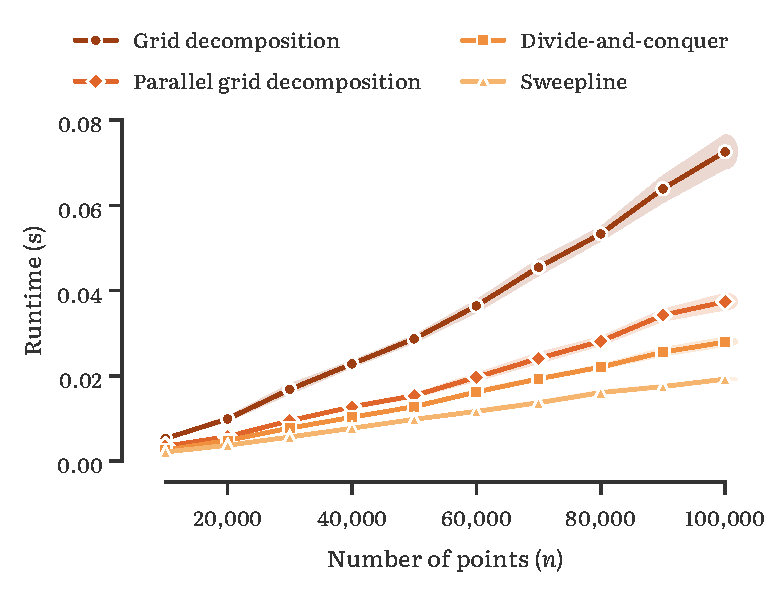
\includegraphics[scale=\figurescale]{diagrams/low_dimensions_two_dimensional_runtime.pdf}
    \caption{Mean runtime of the exact algorithms at $d = 2$. Shaded bands show the 95\% confidence interval of each mean.
    }
    \label{fig:low_dimensions_two_dimensional_runtime}
\end{figure}

\section{Beyond Two Dimensions}

While the two-dimensional algorithms have proven encouraging, both theoretically and empirically,
the real challenge is to solve the problem at higher dimensions, and this is where tools like
divide-and-conquer and sweepline begin to fall apart as you can't easily generalise them.

\subsection{An Attempt to Generalise Sweepline}

To understand why scaling sweepline is hard, let's consider how one might refactor the current
implementation. The core of the issue is to support queries where given some $\delta$ (the
best distance so far), and the current point $(q_{1}, \dots, q_{d})$, we need to find all points such
that along every axis, we have $|p_{i} - q_{i}| < \delta$. In two dimensions, we use a two-pointer
approach to ensure the $x$ axis satisfies this condition, and on the $y$ axis,
we maintain sorting through a balanced binary search tree. Everything hinges on the
two-pointer sweep, because solving one-dimensional range queries is easy.

Let's try to solve range queries for more than two dimensions. For a moment, let's forget
about the two pointers; in just two dimensions, how may we support the range queries? An
esoteric data structure comes to mind: the \textit{Merge Sort Tree}. It's basically a
segment tree on the $x$ values, and each node in the segment tree stores its points sorted
by $y$ values. To answer a query, we perform a binary search on each relevant node, and
there are $\mathcal{O}(\log n)$ of them. Thus, query resolution only costs $\mathcal{O}(\log^{2} n)$.
This idea may be generalised to any dimension; we may put a merge sort tree into
the node of another merge sort tree (in the literature it's known as a \textit{range tree}),
so at dimension $d$ it'll take $\mathcal{O}(\log^{d} n)$ time.

For convenience, let's not bother with point updates, i.e., we'll build the massive
tree once at the start and keep querying it repeatedly. Yes, we're dropping the sweep
out of the sweepline, but ultimately the total time complexity is still an optimistic
$\mathcal{O}(d \cdot n \log^{d} n)$. The limiting factor is no longer time but \textit{memory}. And
since the size of the tree is $\mathcal{O}(d \cdot n \log^{d - 1} n)$, at say $n = 10^{4}$ and
$d = 5$, we have already racked up gigabytes of memory. There's simply no space to
store the data structure!

\subsection{Grid Decomposition (Revisited)}

One neat property of grid decomposition is that it extends naturally to arbitrary dimensions.
A square morphs into a hypercube, and now we need to check adjacent hypercubes instead. There's
one big problem though; at dimension $d$, there are $(3^{d} - 1)/2$ neighbours to check, and
beyond a certain point, you're better off just brute-forcing.

As pessimistic as it sounds, let's try to exploit the nature of the point distribution to
improve the selection of the grid width. Knowing that we have a uniform random distribution,
it's possible to work out how far, on average, a point is from its nearest neighbour, and then
we could use that as a basis for our grid width. This is an ancient problem that was solved
by Hertz in 1909 for points scattered through three-dimensional space~\cite{hertz1909}, and the
same analysis extends to any dimension. For $n$ points spread uniformly through a box of volume $V$, the
expected distance from a point to its nearest neighbour is
\[
    \mathbb{E}[R] = \Gamma\!\left(1 + \frac{1}{d}\right) \left(\frac{V}{n \, \omega_{d}}\right)^{1/d},
\]
where $\omega_{d} = \pi^{d/2} / \Gamma(\sfrac{d}{2} + 1)$ is the volume of a $d$-dimensional ball of
radius $1$, and $\Gamma$ is Euler's \textit{Gamma function}. In our implementation,
\code{unit_ball_volume} supplies $\omega_{d}$, \code{std::tgamma} the Gamma
function, and \code{bounding_box_volume} measures $V$ from the points themselves.
The function \code{expected_nearest_neighbour_distance} then puts
the pieces together.

While it's possible to use this result directly as the grid width, we hesitated to do so and
went with double this expected value instead. One reason is that we don't want to have hypercubes that
are too tiny; with fewer hypercubes, we waste less time on the hash lookups. Another, admittedly
more important, reason is rooted in safety. An expected value is not the same as the actual value;
if we use a grid width that's too small, we end up not finding anything at all, which is even worse.
At small $n$ the variance is too high, and the formula isn't useful, so below
\code{SMALL_POINT_COUNT} we fall back to random sampling.

\begin{aside}
     A more insidious bug caused by grid widths that are too small is reporting the wrong answer.
     Let's say that we have two points $a$ and $b$ on a horizontal line, one at $x = 0.95w$
     and the other at $x = 2.05w$. They have a distance of $1.1w$, though they won't end up
     in adjacent squares. Let's also have a point $c$ at $x = 3.95w$; it'll be paired
     with point $b$ and give a ``best'' distance of $1.9w$, even though we know the true
     minimum is lower. Luckily, with the uniform random distribution such an edge case
     is statistically very unlikely. For guaranteed correctness in arbitrary distributions, stick to
     random sampling.
\end{aside}

\subsection{$k$-dimensional Tree}

A closely related problem to finding the closest pair is to handle point queries where given a
certain point, we ask for the nearest point to it. Answering the main problem then becomes
calling point queries on every point, and if we can perform this point query fast enough, we'll
beat the brute force approach.

As fate would have it, decades ago people already invented a data structure called the $k$-dimensional
tree. In short, each node of this \textit{binary tree} contains a point. To construct the tree,
let's assume we're at the root. To decide which point gets to be the root, we'll take the \textit{median}
point based on the first axis (in two dimensions that'll just be $x$). Now, all points with $x$ less
than the median go to the left subtree and the rest go to the right subtree. Recurse down to
the next subtree and this time, we'll partition based on the second axis (i.e., $y$). Rinse and
repeat till the tree is fully constructed. Note that the maximum depth of this tree might \textit{not}
be $d$, it could exceed $d$ and if so we just loop back to the first axis.

To resolve a query, let us conduct a depth-first search from the root.
At each node in the tree, let's use it to improve the current score. Next, we need to figure
out which subtree is likely to give us a better answer, and the instinct is to use the current
axis as a basis of comparison. For example, if $x$ of our query point is greater than that of the
current node, let's recurse the right subtree. What's important to realise is that this
is just a \textit{heuristic}, it's not guaranteed that the nearest point is going to be in
the right subtree!

Denoting the gap along this axis as $g = x_{q} - x_{m}$, where $x_{q}$ is the $x$ coordinate
of the query point and $x_{m}$ is the $x$ coordinate of the node, and without loss of generality
assume that $g \geq 0$ (the right subtree case), then if $g \geq c_{\text{best}}$, where
$c_{\text{best}}$ denotes the current minimum distance, there's no point exploring the
left subtree since we'll need to pay the cost of $g$ which already exceeds our best answer.

Empirically, this data structure works great on our points because of the underlying uniform
random distribution. During tree construction, we're almost always able to attain two subtrees
of approximately equal size. As a result, the binary tree is very balanced, and the build stage
consumes $\mathcal{O}(n \log n)$ time. Another phenomenon at low dimensions
is that this pruning heuristic cuts off useless subtrees really well, allowing us to enjoy
point queries in roughly $\mathcal{O}(\log n)$ time, leading to a total time complexity of $\mathcal{O}(n \log n)$.
Of course, things break down at higher dimensions because points become sparse,
and the contribution of each dimension towards the overall distance is tinier. Eventually,
we end up needing to search both subtrees. Fortunately, it just degrades to the brute force,
unlike general grid decomposition that mandates searching all neighbouring hypercubes.

\begin{figure}[ht]
    \centering
    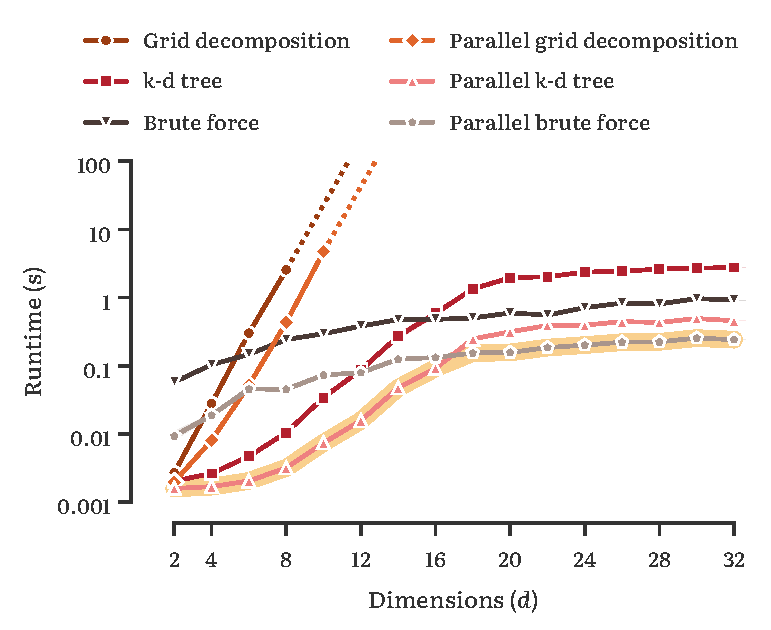
\includegraphics[scale=\figurescale]{diagrams/low_dimensions_runtime_against_dimensions.pdf}
    \caption{Mean runtime at $n = 10{,}000$ as $d$ grows, on a log scale. Grid decomposition stops
        at $d = 8$ and its parallel variant at $d = 10$, as each trial beyond that takes too long.
        The orange highlight traces the fastest algorithm at each $d$.
    }
    \label{fig:low_dimensions_runtime_against_dimensions}
\end{figure}

\begin{aside}
    Given how promising the $k$-dimensional tree is, it'd be sweet if we could somehow
    parallelise it. Between the build and query phases, the latter seems more straightforward
    to parallelise. In fact, because retrieving the closest pair is just making $n$
    queries, we may simply allocate each thread to a set of queries. Though one might
    think it's yet another embarrassingly parallel problem, it turns out there's some nuance
    to it.

    Observe that the smaller the current best distance, the more effective the pruning.
    Decoupling the queries across threads leads to improvements for sure, but the speedup
    isn't as great as we'd expect since the threads can't use the best answer from other
    threads to improve their search. Thankfully, an easy way to share state is through an
    atomic like \code{std::atomic<int64_t>}. The next question is to decide when
    to update this global best. As correct as it appears to update it during recursion,
    putting it in the hot path is likely to hurt more than it helps, even with the
    most lenient memory order, that is, \code{std::memory_order_relaxed}. Therefore,
    we'd rather do a quick update at the end of each point query. Not only do you
    now enjoy extra pruning through the shared global best distance, it comes without
    paying the full price of synchronisation overheads.
\end{aside}

Figure~\ref{fig:low_dimensions_runtime_against_dimensions} pits the various solvers against
each other. Burdened by the curse of dimensionality, grid decomposition is quickly overtaken
by the brute force at small $d$, and parallelising it only buys us so much time. Looking
at the orange highlight, the parallel $k$-dimensional tree is our best bet for $d \leq 16$.
Beyond that, pruning starts to break down, as closeness along one axis does not imply
general proximity, and we end up traversing almost the entire tree instead. Thus, you end
up paying for recursion that offers little benefit, and a simple parallel brute force
is, as anticlimactic as it sounds, the winner.


% !TeX root = main.tex

\chapter{Heuristics}

In the previous chapter, we explored algorithms that found the exact closest pair.
However, at high dimensions, with millions of points, these algorithms become
computationally infeasible. The saving grace is that in many practical applications, we do
not always require the best answer, and can settle for something that is just \textit{good enough}.
As we shall see, even trying out many random pairs finds one that happens to be close to
the closest one. And we can also use simple principles to improve the quality of our guesses,
i.e., \textit{heuristics}. The downside of such techniques is that we cannot prove how
good or bad the final answer is, unlike \textit{approximation algorithms} where we put a limit
on the magnitude of the final error.

To judge the quality of a heuristic algorithm, we can measure how far off the discovered pair is
from the minimum distance. This needs to be handled carefully, however; the more iterations we run
of the random pair guessing algorithm, the more likely it is to get a better answer, so it is not
fair to buff a heuristic simply through stacking more guesses. Let us introduce the idea of a
\textit{budget}, so that each algorithm has a certain ``capacity'', which may be thought of as
a resource to be spent. The implication is that we can fix the budget, and attribute superior performance
to smarter ideas, rather than to more compute.

The most tempting approach would be to have this budget be \textit{runtime}, but empirically, it is not
that easy to figure out the set of parameters that yield a precise runtime. The alternative is
to go with a more theoretical construct, that is, the number of comparisons. Each comparison
is a distance computation between two points, and the budget is the number of comparisons you
perform per point, i.e., total comparisons over $n$. The budget is thus an integral
``multiple'' that is easy to work with. For simplicity, we define the budget rather loosely:
if you examine the same pair twice, it counts twice, and we exclude the cost of precomputations
from this budget, so you may perform sorting or build data structures free of charge. Of course,
the precomputations cannot be ludicrous; the ones used are all of subquadratic time.

\section{Random Pairs}

The simplest heuristic algorithm is born from a tiny modification to the brute force. At each
point, instead of trying every other one of the $n - 1$ points, we will pick a partner uniformly
at random and repeat this $a$ times (\code{attempts_per_point}). The budget is just $a$.

As seen in Figure~\ref{fig:heuristics_random_pairs}, the \textbf{ratio} (i.e., the distance found
divided by the true minimum distance) steadily decreases as we increase $a$. At $a = 60$,
we have found a pair whose distance is about $2.3$ times the closest distance. There
are diminishing returns to increasing $a$; going from $a = 6$ to $18$ improves the mean
by about as much as going from $18$ all the way to $60$. Luck is an important component
too; for each $a$, the ratio spread is pretty wide as we go from trial to trial,
and you could go anywhere from one to four at $a = 60$. Regardless, it is comforting
to know that examining just a tiny fraction of possible pairs already yields such a low ratio.

\begin{figure}[ht]
    \centering
    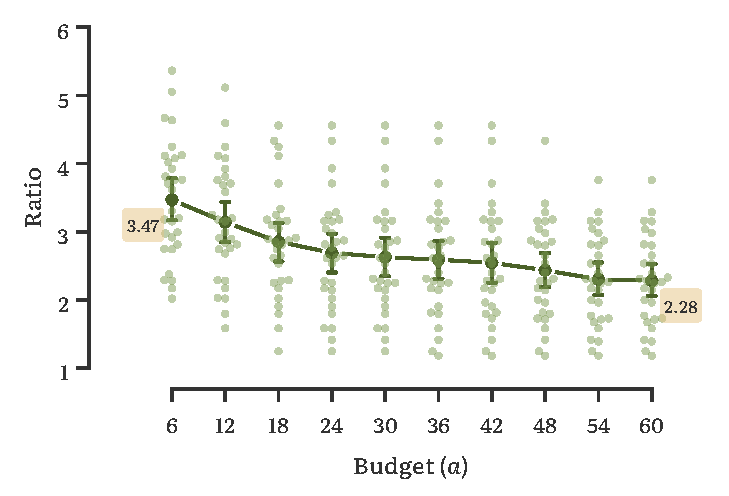
\includegraphics[scale=\figurescale]{diagrams/heuristics_random_pairs.pdf}
    \caption{Random pairs at $d = 6$ and $n = 10{,}000$.}
    \label{fig:heuristics_random_pairs}
\end{figure}

\section{Neighbours in a Sorted Order}

Sorting is the basis of the divide-and-conquer and sweepline algorithms. The reason they do not
scale to high dimensions is that the ``box'' of valid neighbours grows exponentially with $d$.
Nevertheless, there are different heuristics we may use to sort the points, the goal being
to place points that are close to each other near one another in the sorted order.

\subsection{Along Each Axis}

The first idea that comes to mind is to sort the points using their coordinate on one axis,
and then apply a sliding window, i.e., check $w$ neighbours per point. Intuitively, a closest pair
should be close on some axis (though there are counterexamples to refute this), and in total we
have a budget of $d \cdot w$.

\subsection{Along Random Directions}

To generalise the earlier idea, we can actually create our own axis (so we unlock
an arbitrary number of directions to sort by). First, let us pick some direction 
$u$ in $d$-dimensional space. Each component of $u$ is drawn independently from a standard normal
distribution, which makes the direction uniformly random over all directions~\cite{muller1959}.
Next, every point $p$ gets a sort key equal to the \textit{projection} $p \cdot u$. The
total budget is $m \cdot w$ (where $m$ is captured by \code{direction_count}).

\begin{figure}[ht]
    \centering
    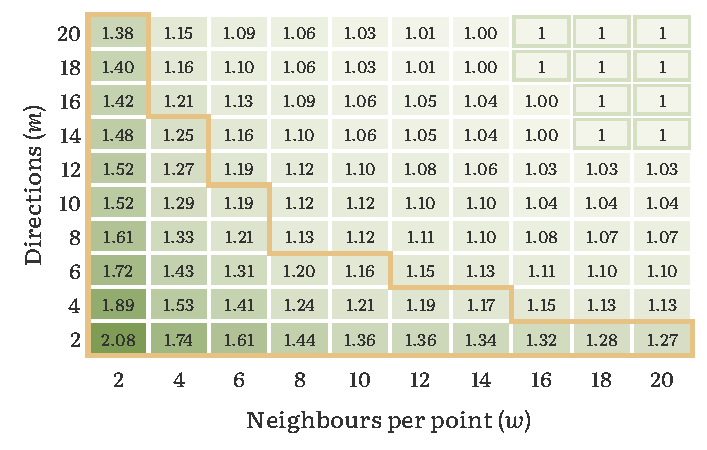
\includegraphics[scale=\figurescale]{diagrams/heuristics_random_directions.pdf}
    \caption{Mean ratio of random directions at $d = 6$ and $n = 10{,}000$; the yellow-bordered
        zone represents cells where $m \cdot w \leq 60$. Cells marked $1$ found the
        distance of the closest pair in \textit{every} trial.
    }
    \label{fig:heuristics_random_directions}
\end{figure}

As Figure~\ref{fig:heuristics_random_directions} shows, sorting is truly a powerful tool. Even
at a budget of four, we have already surpassed the best ratio random pairs had to offer at a budget
of sixty. In fact, given a maximum budget of sixty, trying random directions nets us a best ratio
of $1.16$.

Between $m$ and $w$, $w$ appears to have a slightly larger contribution, but that is
not to say $m$ is useless, because trying more directions reduces the risk of unlucky projections.
Another noteworthy observation is that at a budget of around three hundred, we are even able to
find the global minimum.

\subsection{Along the Z-order Curve}

An unorthodox way to sort would be through the Z-order curve (or Morton order~\cite{morton1966}).
This is a path that goes through every cell of a grid, and it forms a Z shape, giving it its
name. A point's position on the curve comes from \textit{interleaving} the bits of its coordinates:
starting from the topmost bit, you take one bit from each axis in turn. For example, $x = 101_{2}$
and $y = 011_{2}$ interleave to $100111_{2}$.

\begin{figure}[ht]
    \centering
    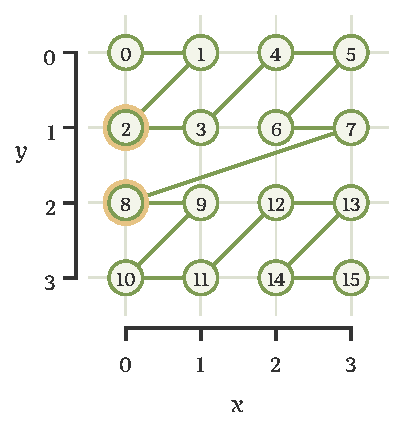
\includegraphics[scale=\figurescale]{diagrams/heuristics_z_order.pdf}
    \caption{The Z-order curve on a $4 \times 4$ grid. The two highlighted points are close on the
        grid, but far apart on the curve.
    }
    \label{fig:heuristics_z_order}
\end{figure}

\begin{aside}
    The most direct method to compare two points is to literally build the interleaved value.
    Since coordinates take up to $30$ bits, the resulting value would have $30 \cdot d$ bits,
    which does not fit in native types for many $d$. However, we only really care about
    the highest bit where the two points differ; a trick to check whether $x$ has a lower top
    bit than $y$ (\code{has_lower_most_significant_bit}) is to test $x < y$ and
    $x < x \oplus y$, where $\oplus$ is bitwise exclusive-or~\cite{chan2002}.
\end{aside}

As is evident from Figure~\ref{fig:heuristics_z_order}, points $\bigl(\begin{smallmatrix} 0 \\ 1 \end{smallmatrix}\bigr)$
and $\bigl(\begin{smallmatrix} 0 \\ 2 \end{smallmatrix}\bigr)$ are
close in terms of Euclidean distance, but when inspected in Morton order, they end up far
apart. One remedy is to apply a random shift to every point, creating a new order in the process.
Implementation-wise, we refrain from adding a shift to the very first order; only later orders
get a fresh shift, applied independently to each axis. With $s$ orders, we have a total budget
of $s \cdot w$.

\begin{figure}[ht]
    \centering
    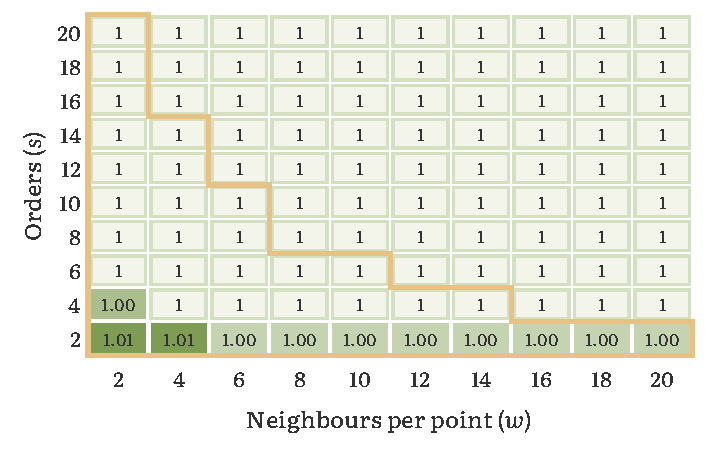
\includegraphics[scale=\figurescale]{diagrams/heuristics_z_order_heatmap.pdf}
    \caption{Mean ratio of the Z-order curve at $d = 6$ and $n = 10{,}000$; the yellow-bordered
        zone represents cells where $s \cdot w \leq 60$.
    }
    \label{fig:heuristics_z_order_heatmap}
\end{figure}

The Z-order curve is staggeringly impressive. Figure~\ref{fig:heuristics_z_order_heatmap} reveals
that across almost the entire budget spectrum, the closest pair was found \textit{thirty out of thirty}
times. Only with the fewest orders does the Z-order curve sometimes trip up and find a slightly
suboptimal pair.

\section{Best-first Search on the $k$-dimensional Tree}

In light of the success of the $k$-dimensional tree in the previous chapter,
it seems plausible that we could exploit the structure of the tree to reach nearby
points early in the traversal. Let us test out this
hypothesis by limiting the number of nodes traversed per query to just $b$. To pick the nodes
for expansion, we can use a Dijkstra-like approach (i.e., a best-first search) with
a min-heap. The budget is just $b$.

\begin{figure}[ht]
    \centering
    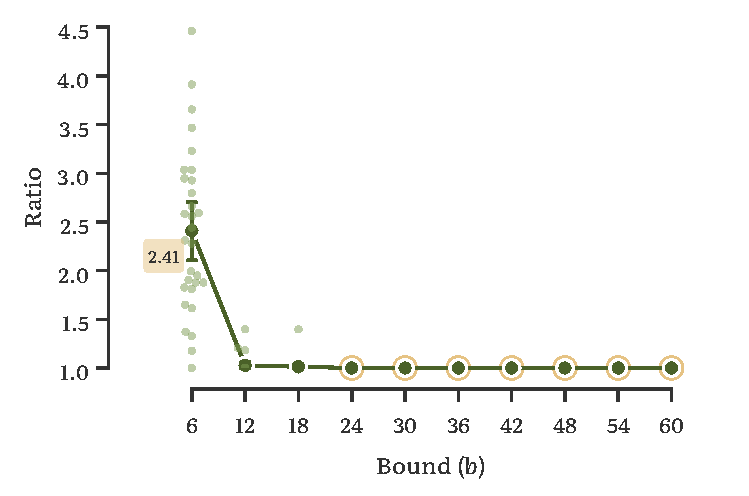
\includegraphics[scale=\figurescale]{diagrams/heuristics_best_first.pdf}
    \caption{Best-first search at $d = 6$ and $n = 10{,}000$; yellow rings mark the bounds where
        \textit{every} trial found the distance of the closest pair.
    }
    \label{fig:heuristics_best_first}
\end{figure}

It is apparent from Figure~\ref{fig:heuristics_best_first} that the results are on par
with the Z-order curve. At $b = 6$, the ratio is not particularly
great, but that is because traversal always begins from the root, regardless of the
query, and there will always be a few ``wasted nodes'' that cannot be avoided as part
of the expansion process. Nevertheless, from $b = 24$ onwards, it consistently
discovers the closest pair.

\section{High Dimensions}

As helpful as the ratio has been in our earlier benchmarking process, this metric
begins to lose its effectiveness at higher dimensions. At low dimensions, our best
heuristic algorithms are getting perfect scores, and at high dimensions, we are
\textit{also} getting near-perfect scores, which should raise some suspicions. The
reason is that the distribution of pair distances begins to contract as we increase the
number of dimensions, and even random pairs yield tiny ratios at high dimensions
(Figure~\ref{fig:heuristics_high_dimensions}).

\begin{figure}[ht]
    \centering
    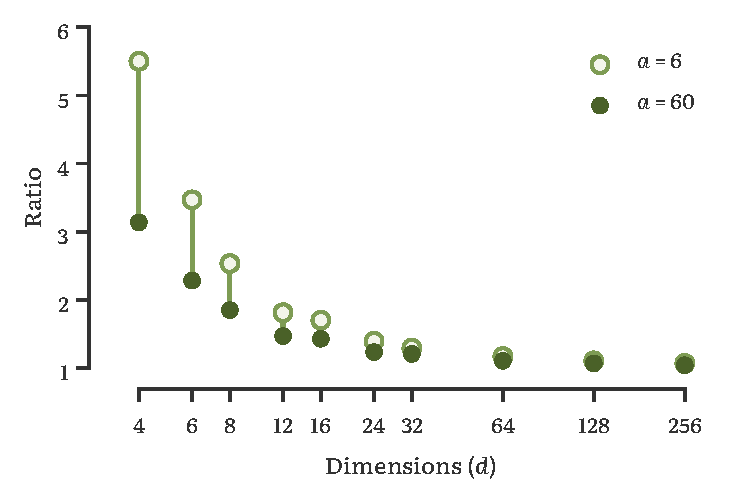
\includegraphics[scale=\figurescale]{diagrams/heuristics_high_dimensions.pdf}
    \caption{Mean ratio of random pairs at $n = 10{,}000$ as $d$ grows, at $a = 6$
        and $a = 60$.
    }
    \label{fig:heuristics_high_dimensions}
\end{figure}

Because the ratio only compares our pair with the closest pair, it fails to carry any information
about the underlying distribution. As $d$ grows, almost all pairs are about equally far apart,
a phenomenon known as \textit{distance concentration}~\cite{beyer1999}. He et al.\ measure this with
\textit{relative contrast}: the mean distance from a query to the data, divided by the distance
to its nearest neighbour~\cite{he2012}. Building on this idea, let $\delta$ be the distance
of the closest pair, $t$ be the mean distance over all pairs, and $x$ be the distance of a
candidate pair. We define the normalised score as:

\[
    S = \frac{t - x}{t - \delta}
\]

Visualise it as a ruler; your average pair lies at $0$ and the closest pair at $1$. This metric
does have a weakness, however, in that at low dimensions, because the ``ruler'' is incredibly
long, almost any pair scores pretty well.

As anticipated, Figure~\ref{fig:heuristics_comparison} reveals that even the strongest heuristic
algorithms have their limits. Performance-wise, the Z-order curve and best-first search are clearly
the (tied) winners. Random directions holds its own at $d \leq 8$, but its normalised score plummets
after that. There are three trends worth noticing. First, the normalised score tends to decrease
across the board as $d$ increases; as we enter sparse territory it becomes harder to leverage
data structures or representations that put close points beside each other. Second, the
\textit{variance} of the normalised score also rises with $d$ before levelling off at around
$d = 64$, i.e., it becomes harder to hit the mean score consistently. Finally, all four techniques appear
to converge to the same performance eventually. At super high dimensions, ``cleverness'' does not help
much and you are no better off than just trying random pairs. As pessimistic as it sounds, 
heuristics still have real value in commonly encountered dimensions. After all, it is not often one
needs to work with $2048$ dimensions,
and even at convergence, getting $90\%$ of the way there by examining about $2.6\%$ of the pairs is still
worth the compute.

\begin{figure}[ht]
    \centering
    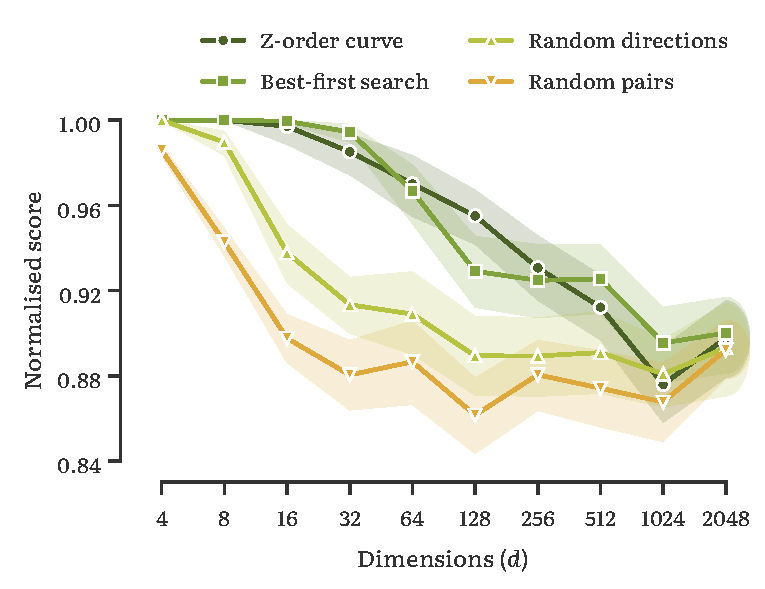
\includegraphics[scale=\figurescale]{diagrams/heuristics_comparison.pdf}
    \caption{Mean normalised score at a budget of $128$ and $n = 10{,}000$, using $s = 8$, $w = 16$ for
        the Z-order curve, $b = 128$ for best-first search, $m = 8$, $w = 16$ for random directions,
        and $a = 128$ for random pairs. Shaded bands show the 95\% confidence interval of each mean.
    }
    \label{fig:heuristics_comparison}
\end{figure}


% !TeX root = main.tex

\chapter{Approximations}


\bibliographystyle{plainurl}
\bibliography{references}

\end{document}
